\documentclass[a4paper,12pt]{report}
\usepackage[top=1in, bottom=1in, left=1in, right=1in]{geometry} % Custom margins
\usepackage[dutch]{babel}
\usepackage[T1]{fontenc} % Special chars
\usepackage[section]{placeins}
\usepackage{float}
\usepackage{graphicx} % \includegraphics
\graphicspath{{./img/}}
\usepackage[hidelinks]{hyperref} % \url
\usepackage{pdfpages} % \includepdf
\usepackage{tocbibind} % Custom toc entries
\usepackage{listings} % Code snippets
\lstdefinestyle{code}{
  basicstyle=\ttfamily\footnotesize,
  breakatwhitespace=false,         
  breaklines=true,                 
  captionpos=b,                    
  keepspaces=true,                 
  numbers=left,                    
  numbersep=5pt,                  
  showspaces=false,                
  showstringspaces=false,
  showtabs=false,                  
  tabsize=2
}
\lstset{style=code}
\usepackage{blindtext} % Lorem ipsum
\usepackage[backend=biber,style=apa]{biblatex} % References
\addbibresource{references.bib}

\title{Implementatie van een NIDS binnen een ISP omgeving}
\author{Jonas Meeuws}

\begin{document}

% Bedrukte kaft (=titelblad)

\includepdf[pages=-]{./include/titelblad.pdf}

% Schutblad
\newpage
\thispagestyle{empty}
\mbox{}

% Titelblad

\includepdf[pages=-]{./include/titelblad.pdf}

% Mededeling
\chapter*{Mededeling}
\addcontentsline{toc}{chapter}{Mededeling}
Deze eindverhandeling was een examen.
De tijdens de verdediging geformuleerde opmerkingen werden niet opgenomen.

% Woord vooraf (niet verplicht)
\chapter*{Woord vooraf}
\addcontentsline{toc}{chapter}{Woord vooraf}
% Hier heb je de mogelijkheid om je waardering uit te drukken en dank te betuigen. Je neemt in
% het woord vooraf geen gegevens op die essentieel verband houden met het behandelde
% onderwerp (methode, doelstelling, enz.).
\blindtext

% Samenvatting of abstract
\chapter*{Samenvatting}
\addcontentsline{toc}{chapter}{Samenvatting}
\blindtext

% Inhoudsopgave
\tableofcontents
\newpage

% Lijst van figuren (niet verplicht)
\listoffigures

% Inleiding
\chapter*{Inleiding}
\addcontentsline{toc}{chapter}{Inleiding}
\blindtext

% Inhoud
\chapter{Intrusion detection}
Intrusion detection is het monitoren van systemen op verdachte activiteit.
Dit omvat pogingen tot hacken, verspreiding van virussen of malware, aanwezigheid van rogue devices\dots

Intrusion detection gebeurt typisch volledig passief.
De logs die een IDS (Intrusion detection system) produceert kunnen worden verstuurd naar een administrator als een alert.
In grotere systemen worden deze logs centraal verzameld om deze anomalieën effectief te kunnen analyseren.
\autocite{wikipedia:ids}

Intrusion detection systemen worden opgedeeld in 2 soorten: network (NIDS) en host (HIDS) intrusion detection.

\section{NIDS}
Een network intrusion detection systeem (NIDS) monitort een netwerkverbinding.

De 2 grote NIDS software projecten zijn Snort en Suricata.
Voor een groot deel werken de 2 systemen identiek voor een eindgebruiker.
Zo is de NIDS rule syntax van Snort en Suricata bijna gelijk.
Het verschil ligt in specifieke features.
Voorbeelden van features die enkel beschikbaar zijn in Suricata zijn detectie van meer protocollen, bestanden opslaan uit http/ftp/smtp, lua scripting\dots
Alle verschillen staan duidelijk beschreven in de documentatie van Suricata.
\autocite{suricata:docs}

\subsection{Regels}
Een NIDS monitort gecapteerd netwerkverkeer aan de hand van een lijst van regels.
Deze regels volgen een bepaalde syntax.

Een voorbeeld van een nids rule is als volgt (figuur \ref{fig:nids-rule}).

\begin{figure}[H]
  \begin{lstlisting}
alert tcp $EXTERNAL_NET any -> $INTERNAL_NET 3306 (msg:"Inbound SQL connection"; sid:1000000;)
  \end{lstlisting}
  \caption{Een voorbeeld van een nids rule}
  \label{fig:nids-rule}
\end{figure}

Deze rule zorgt ervoor dat er een alert wordt gegenereerd wanneer de NIDS engine een tcp verbinding ziet van het extern netwerk naar het intern netwerk op poort 3306.
Het extern netwerk is meestal het internet of een WAN, het intern netwerk is meestal een LAN.
Volgens het tcp client-server model is de client een externe host en de server een interne host.

Poort 3306 is gereserveerd voor MySQL database verbindingen \autocite{iana:ports}.
Deze verbindingen kunnen perfect normaal zijn als de client een vertrouwde host is.
In dit geval is de client echter een externe host die acties probeert uit te voeren op een interne MySQL database.
Dit is verdachte activiteit, vandaar het type alert.

\subsection{Variabelen}
Om regels zo effectief mogelijk te maken, worden er variabelen geïntroduceerd.

De 2 meest gebruikte variabelen zijn het \lstinline|INTERNAL_NET| en het \lstinline|EXTERNAL_NET|.
Bijna alle regels gebruiken minstens 1 van deze variabelen, daarom is het van groot belang om deze in te stellen.
Als een variabele niet ingesteld is, worden regels die deze variabele gebruiken genegeerd.

Variabelen kunnen ook de waarde \lstinline|any| aannemen.
Dit kan zorgen voor veel false alerts, maar is wel nuttig in gesloten netwerken waar incidenten zich enkel intern afspelen.

\subsection{Rulesets}
NIDS rules worden gecompileerd in lijsten die makkelijk te gebruiken zijn met een NIDS engine.
Deze lijsten worden onderhouden door bedrijven en online gemeenschappen.

Een voorbeeld van een ruleset is Emerging Threats (van \url{https://rules.emergingthreats.net/}).
Deze wordt dagelijks geüpdatet met nieuwe en aangepaste rules.
Een klein stuk van de ruleset staat in figuur \ref{fig:et-voorbeeld}.
Het volledige bestand bevat momenteel bijna $30000$ lijnen.

Sommige bedrijven hebben ook \emph{subscription-based} rulesets.
De officiële Snort ruleset (\url{https://www.snort.org/}) volgt zo'n model.
Updates aan de ruleset worden meteen beschikbaar gemaakt aan subscribers, 30 dagen later worden dezelfde veranderingen ook toegepast op een vrije versie van de ruleset.
Niet-betalende gebruikers hebben dus steeds een versie die 30 dagen ouder is.

\begin{figure}[H]
  \begin{lstlisting}[basicstyle=\ttfamily\scriptsize]
...
alert tcp $SQL_SERVERS 1433 -> $EXTERNAL_NET any (msg:"GPL SQL sa brute force failed login attempt"; flow:from_serv...
alert tcp $SQL_SERVERS 1433 -> $EXTERNAL_NET any (msg:"GPL SQL sa brute force failed login unicode attempt"; flow:f...


# ----- Begin ET-emerging-telnet Rules Category ----- #

# -- Begin GID:1 Based Rules -- #

alert tcp $HOME_NET 23 -> $EXTERNAL_NET any (msg:"ET TELNET External Telnet Attempt To Cisco Device With No Telnet ...
#alert tcp $HOME_NET 23 -> $EXTERNAL_NET any (msg:"ET TELNET External Telnet Login Prompt from Cisco Device"; flow:...
alert tcp $EXTERNAL_NET any -> $HOME_NET [23,2323,3323,4323] (msg:"ET TELNET SUSPICIOUS Path to BusyBox"; flow:to_s...
#alert tcp $EXTERNAL_NET any -> $HOME_NET [23,2323,3323,4323] (msg:"ET TELNET SUSPICIOUS busybox shell"; flow:to_se...
#alert tcp $EXTERNAL_NET any -> $HOME_NET [23,2323,3323,4323] (msg:"ET TELNET SUSPICIOUS busybox enable"; flow:to_s...
...
  \end{lstlisting}
  \caption{Een klein stuk van de Emerging Threats ruleset}
  \label{fig:et-voorbeeld}
\end{figure}

\subsection{Port mirror}
Een NIDS engine zoals Snort of Suricata wordt normaal gebruikt om te capteren op 1 netwerkinterface.
Deze interface ontvangt typisch een kopie van een punt in het netwerk.
Dit noemt men een port mirror.

Een voorbeeld van een technologie die port mirroring toelaat is SPAN.
Deze is aanwezig in bijvoorbeeld een switch en kopieert alle pakketten van een source poort naar een destination poort.
Daarnaast kan RSPAN gebruikt worden om gecapteerde pakketten over een laag 2 netwerk te transporteren.
Ten slotte kan ERSPAN op de zelfde manier gebruikt worden om een port mirror te transporteren over een laag 3 netwerk.
\autocite{cisco:span}

Het geheel van een NIDS engine die al het netwerkverkeer op 1 punt in een netwerk capteert, noemt men een sensor.
Eén of meerdere sensoren kunnen in een netwerk geplaatst worden op strategische punten.
Dit zijn vaak plaatsen waar een vertrouwd netwerk wordt verbonden met een extern netwerk.

De meest interresante plaats om een sensor te plaatsen in een bedrijfsnetwerk is meestal de plaats waar NAT toegepast wordt.
Dit is omdat alle communicatie met externe netwerken doorheen dit punt passeert.
Als zo'n sensor aan de buitenkant van de NAT staat, zijn de interne ip-adressen niet zichtbaar.
We zien enkel ip-communicatie tussen de NAT-pool en externe netwerken, zo gaat er veel informatie verloren.
Daarom gaat de voorkeur naar het plaatsen van de sensor aan de binnenzijde van de NAT.

Waar men ook voor moet uitkijken bij het plaatsen van een sensor is of de hardware de bitsnelheid wel aankan.
Als de link tussen de port mirror en de sensor een lager maximum bits/s heeft dan bitsnelheid van de combinatie van de beide richtingen van de te capteren poort, kan er packet loss optreden.
NIDS engines kunnen hiermee wel overweg, maar het zorgt natuurlijk voor verlies van informatie.

\section{HIDS}
Een host intrusion detection systeem (HIDS) montiort één machine op verdachte activiteit.
Enerzijds wordt dit gedaan door alle data die door de netwerkinterfaces gaat te inspecteren.
Daarnaast wordt het gedrag van processen op de machine bekeken.
\autocite{wikipedia:hids}

Een HIDS komt in de vorm van een \emph{agent} die geïnstalleerd wordt op elke machine, zowel servers als workstations.
Deze agents kunnen verslag uitbrengen naar een centrale applicatie waar incidenten verder verwerkt worden.
In sommige gevallen kunnen de agents ook zelf actie ondernemen, door bijvoorbeeld processen te beëindigen of netwerk poorten te blokkeren.
Voorbeelden van HIDS agents zijn OSSEC, Wazuh, Elastic Beats en Sysmon.

Tijdens deze stage en bachelorproef heb ik geen HIDS gebruikt.
Veel HIDS agents zijn wel compatibel met dezelfde technologieën die NIDS beheren, zoals Security Onion.

\chapter{Security Onion}
\section{Wat is Security Onion?}
De officiële site beschrijft Security Onion als:
``Security Onion is a free and open source Linux distribution for intrusion detection, enterprise security monitoring, and log management.
It includes Elasticsearch, Logstash, Kibana, Snort, Suricata, Zeek, Wazuh, Sguil, Squert, CyberChef, NetworkMiner, and many other security tools.''
\autocite{so:docs}

\section{Geschiedenis}
In 2008 begon Doug Burks met het ontwikkelen van Security Onion.
Een eerste versie van het project werd gepubliceerd in 2009.
Omdat de Linux distributie meer populariteit kreeg, werd het in 2012 volledig herschreven met het doel om performantie en schaalbaarheid te verbeteren.
In 2014 werd Security Onion Solutions LLC opgericht om professionele ondersteuning aan te bieden aan bedrijven.
Met jaarlijkse conferenties bleef het project groeien.
\autocite{so:sos}
In 2018 begon de ontwikkeling van een nieuw project, Security Onion Hybrid Hunter.
Hybrid Hunter is nog steeds in experimentele staat, en het wordt afgeraden dit systeem te gebruiken in een productieomgeving.

\section{Features}
Security Onion heeft veel te bieden om een goed inzicht te krijgen grote hoeveelheden netwerkverkeer waar standalone tools als Suricata of Wireshark te onoverzichtelijk worden.

\subsection{NIDS}
Als een deels afgesloten systeem is er NIDS.
Dit bestaat uit een NIDS engine, ofwel Snort ofwel Suricata, die binnenkomende pakketten vergelijkt met een lijst van rules en al dan niet een alert van bepaalde prioriteit genereert.
Die alerts worden verzonden naar beide Logstash en Sguild.

In Logstash worden de alerts behandeld als logs.
Deze logs zijn dan zichtbaar in Elasticsearch en Kibana.

Sguild is een database voor IDS alerts.
De frontend tools Sguil en Squert voeren queries uit op deze database om de alerts aan de analyst te presenteren.

De HIDS info van OSSEC is ook zichtbaar in beide Elasticsearch en Sguild, maar dit is standaard beperkt tot de OSSEC daemons die op de Security Onion servers zelf opereren.

Mijn voorkeur van NIDS engine gaat naar Suricata, vooral omdat het moderner is.
Suricata heeft afgewerkte ondersteuning voor multithreading en naar mijn mening betere documentatie.

Bij het analyseren van alerts heb ik vooral Squert gebruikt.
Opnieuw is dit een veel gebruiksvriendelijkere en moderne tool dan Sguil.
Sguil heeft wel bepaalde mogelijkheden die ontbreken bij Squert zoals het manueel uitvoeren van SQL queries op de Sguild database.

\subsection{Zeek}
Security Onion definieert een sensor als een verzameling van services die actief zijn op 1 netwerkinterface.
Alle configuratie voor 1 zo'n sensor bevindt zich in een map \lstinline|/etc/nsm/[hostname]-[interface]|.
Naast Suricata of Snort (de NIDS engine) is er nog een andere service die de gecapteerde pakketten analyseert.
Deze service is Zeek.

Zeek (vroeger Bro) is een open-source analyser voor netwerkverkeer.
Van de officiële documentatie:
``Zeek is a passive open-source network traffic analyzer.
It is primarily a security monitor that inspects all traffic on a link in depth for signs of suspicious activity.
More generally, however, Zeek supports a wide range of traffic analysis tasks even outside of the security domain, including performance measurements and helping with trouble-shooting.''
\autocite{zeek:docs}

Zeek heeft de mogelijkheid om gedetailleerde logs te genereren van veel verschillende soorten netwerkverkeer.
Bij tcp verbindingen wordt er bijvoorbeeld bijgehouden wat de source en destination poort was, hoeveel data er uitgewisseld is geweest en hoe de verbinding beëindigd werd.
Udp en icmp pakketten worden gelijkaardig behandeld.
Bij applicatielaag protocollen worden er veel details gehaald uit de plain-text protocollen zoals HTTP, FTP, DNS, MySQL\dots
Ook geëncrypteerde protocollen die SSL gebruiken worden geanalyseerd op \emph{self-signed} en verlopen certificaten.

Enkele velden komen in bijna elke log voor, zoals het source en destination ip-adres.
Hierdoor is het mogelijk om snel correlaties te vinden in verschillende logs met een tool als Kibana.

Deze logs zijn beschikbaar in json-formaat in \lstinline|/nsm/bro/logs|.
De logs worden geconsumeerd door syslog-ng.
Daarna komen ze terrecht in de ELK stack, waar er meer informatie wordt toegevoegd en ze uiteindelijk zichtbaar zijn in Kibana.
\autocite{so:docs}

\subsection{ELK stack}
ELK staat voor Elasticsearch, Logstash, and Kibana.
De ELK stack is een open-source systeem voor het beheren en visualiseren van data (logs) van meerdere bronnen.

Logstash neemt data binnen van verschillende bronnen zoals NIDS, HIDS en Zeek, verrijkt deze bronnen met bijvoorbeeld links naar de volledige pcap files en slaat deze logs op in elasticsearch.
Elasticsearch heeft een uitgebreide api om allerlei soorten zoekopdrachten uit te voeren op deze logs.
Een analyst kan dan de browser gebaseerde tool Kibana gebruiken om de logs in elasticsearch te visualiseren.
\autocite{elastic:what-is-elk}

Security Onion voorziet uitgebreide logs in elasticsearch die alle informatie van NIDS, HIDS en Zeek omvatten.
In Kibana zijn er een 40-tal dashboards aanwezig met in totaal zo'n 400 visualisaties.
Dit is zeker de meest handige tool voor een analyst, Kibana stond aan de kern van elke analyse die ik uitvoerde.

\subsubsection{ElastAlert}
In Security Onion is de service \emph{ElastAlert} voorgeïnstalleerd.
ElastAlert is third-party software die samenwerkt met Elasticsearch.

Met ElastAlert is het mogelijk om alerts te genereren wanneer er nieuwe data binnenkomt in Elasticsearch die overeenkomt een vooraf ingestelde filter.
De combinatie van Elasticsearch indexes, een filter en een methode om alerts te genereren noemt men een \emph{ElastAlert rule}.
Er kunnen zoveel rules aangemaakt worden als men wenst.

Filters kunnen complexe pattronen zijn of elke match doorlaten.
Deze `any' filter is nuttig om alle relevante data te sturen naar een extern systeem.
Dit is de manier waarop TheHive en Security Onion verbonden kunnen worden.
Bij complexe filters met pattronen die zelden voorkomen kan het handig zijn om dit te melden aan een administrator bijvoorbeeld via de Slack alerter.
Figuur \ref{fig:elastalert-slack} is een screenshot van een Slack workspace die ik aanmaakte om enkele filters uit te testen.

\begin{figure}[H]
  \centering
  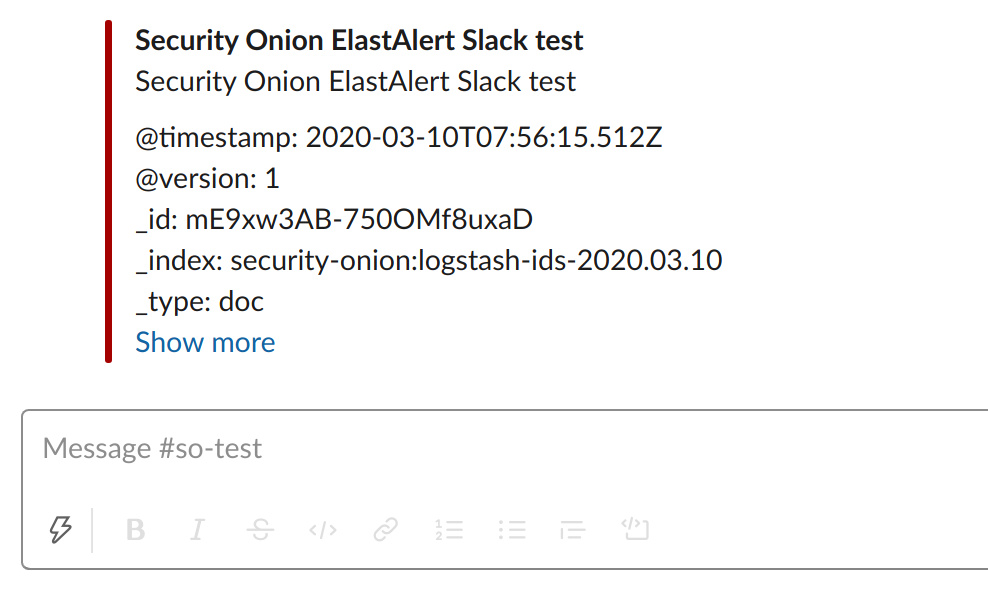
\includegraphics[width=0.8\textwidth]{elastalert-slack}
  \caption{Screenshot van de ElastAlert Slack alerter in een Slack channel}
  \label{fig:elastalert-slack}
\end{figure}

\section{Deployment scenario's}
Security Onion kan op verschillende manieren geïnstalleerd worden.
Dankzij de architectuur van het gehele systeem kunnen bepaalde taken weggenomen worden van de ene server, zodat een andere server met meer geschikte hardware deze taken kan behandelen.
Dit proces noemt men offloading.

\subsection{Evaluation Mode}
Een eerste mogelijkheid is \emph{Evaluation Mode}.
Deze is ideaal om de distributie te verkennen zonder het volledig te installeren in een productieomgeving, maar ook om pcap bestanden offline te analyseren met de kracht van het volledige systeem.

\subsection{Standalone Production Mode}
Een tweede mogelijkheid die beter geschikt is voor permanente opstellingen is de \emph{Standalone Production Mode}.
Hierbij werkt het volledige systeem vanaf 1 server: zowel de sensor, log management, opslag als de web interface vinden plaats op dezelfde \emph{Master node}.
Zie figuur \ref{fig:so-architecture-standalone} voor een schema.
\begin{figure}[H]
  \centering
  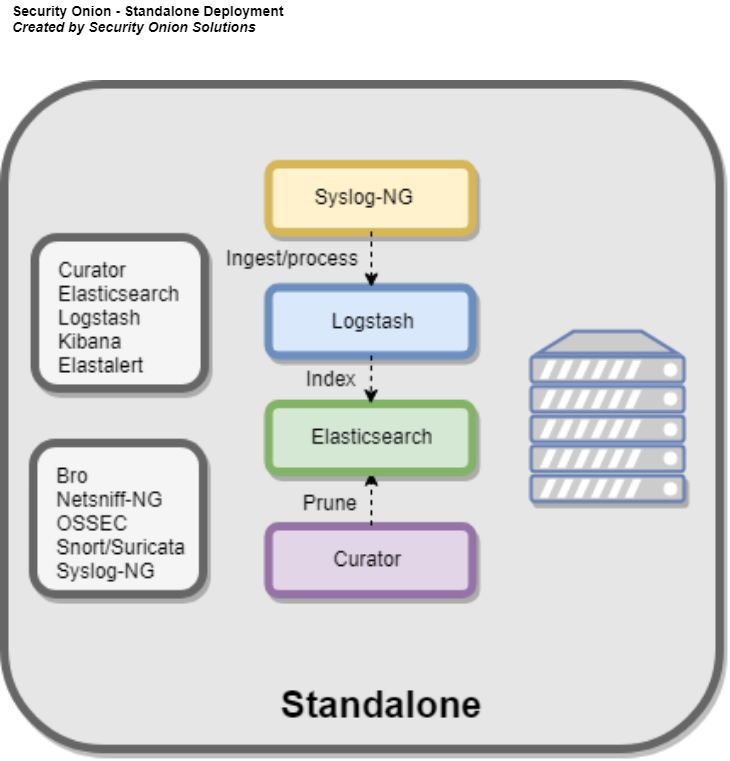
\includegraphics[width=0.5\textwidth]{so-architecture-production-standalone}
  \caption{Standalone Production deployment \autocite{so:docs}}
  \label{fig:so-architecture-standalone}
\end{figure}

\subsection{Distributed Production Mode}
Het laatste mogelijke scenario bestaat uit meerdere nodes met elk een unieke rol.
Zie figuur \ref{fig:so-architecture-distributed} voor een schema.

Elke node heeft standaard een OSSEC daemon actief.
Deze dient om aan Host-based intrusion detection te doen op het Security Onion systeem zelf.

\subsubsection{Forward node}
Een \emph{Forward node} bezit alle functies van een sensor.
Op elke forward node worden er 1 of meerdere port mirrors geïnstalleerd.
De gecapteerde pakketten worden door enkele services verwerkt: Netsniff-NG voor full packet capture, Zeek protocol decoding en Snort of Suricata als NIDS engine.
Alle logs die Zeek en Suricata of Snort genereren worden meteen doorgestuurd naar de Logstash instantie op de master server.
De full packet capture van netsniff-ng, blijft echter op de forward node aanwezig.
Deze pcap files kunnen opgehaald worden wanneer ze nodig zijn en worden automatisch verwijderd wanneer er te weinig vrije plaats is op de disk.

Door meerdere forward nodes strategisch te plaatsen in een netwerk, kan er veel beter inzicht verkregen worden in het netwerk.

\subsubsection{Master node}
De master node is standaard verantwoordelijk voor alle andere taken die geen raw pcap data verwerken.
Log management services zoals Elasticsearch, Logstash en Sguild zijn hier actief en frontend applicaties voor de analyst zoals Kibana en Squert worden hier gehost.

\subsubsection{Storage node}
Storage nodes kunnen gebruikt worden om de opslagcapaciteit uit te breiden en het verwerken van logs te verlichten voor de master node.

\subsubsection{Heavy node}
Heavy nodes zijn een combinatie van storage nodes en forward nodes.
Deze worden afgeraden om te gebruiken, maar kunnen wel gebruikt worden wanneer forward en storage nodes niet gesplitst kunnen worden omwille van bijvoorbeeld beperkte hardware.

\autocite{so:docs}

\begin{figure}[H]
  \centering
  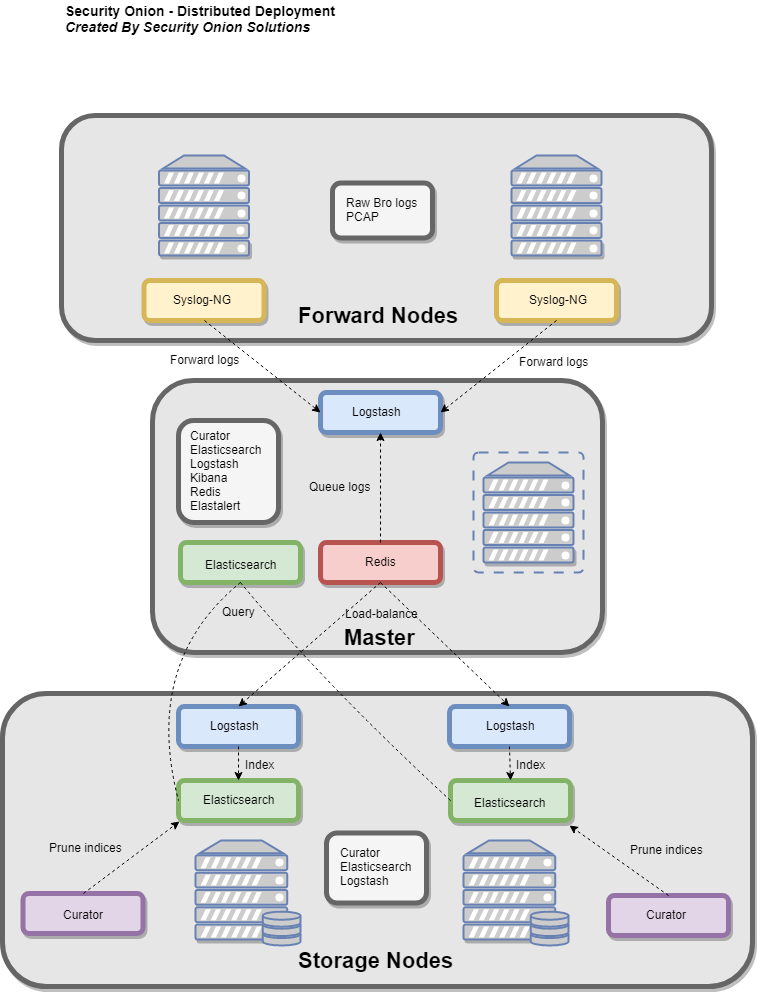
\includegraphics[width=0.6\textwidth]{so-architecture-production-distributed}
  \caption{Distributed Production deployment \autocite{so:docs}}
  \label{fig:so-architecture-distributed}
\end{figure}

\chapter{Opstelling}
\section{Simulaties met GNS3}
% GNS3 uitleggen
GNS3 is een open source softwarepakket waarmee netwerken gesimuleerd kunnen worden via een grafische interface.
De reden dat GNS3 aantrekkelijk leek om tijdens de stage te gebruiken, was omdat het niet enkel routers en switches ondersteunt, maar ook virtuele machines.
Op die manier kon ik simulaties maken van netwerken bestaande uit Securty Onion nodes en bijvoorbeeld Kali Linux en Ubuntu hosts.

Ook is het troubleshooten en leren hoe Security Onion netwerk verkeer interpreteert veel makkelijker met GNS3.
Op elke netwerkverbinding kan een \emph{capture sessie} gestart worden waarbij bijvoorbeeld Wireshark geopend wordt.
Zo kan alle data op het netwerk live bekeken worden.

Voor kleine simulaties kan GNS3 rechtsreeks op een laptop of desktop uitgevoerd worden.
Dit vereist wel dat er andere software geïnstalleerd is voor het uitvoeren van alle verschillende gesimuleerde devices. 
Om Docker containers te gebruiken in een netwerk moet Docker geïnstalleerd zijn, voor de meeste virtuele machines moet QEMU geïnstalleerd zijn\dots
\autocite{gns3:home}

Voor grote opstellingen of om de installatie makkelijker te maken is er ook een officiële GNS3 VM image.
Deze kan door een virtuele machine als besturingssysteem gebruikt worden en bevat de GNS3 server met alle vereiste software of \emph{dependencies}.
Merk op dat geneste virtualisatie beschikbaar moet zijn om virtuele machines uit te voeren in de GNS3 virtuele machine.
Een GNS3 client (de grafische applicatie) kan dan verbinden met de server in de GNS3 VM.

Voor de stage begon had ik Security Onion al uitgeprobeerd aan de hand van GNS3 op mijn desktop.
In het begin van de stage kreeg ik toegang tot een virtuele machine met de GNS3 VM image geïnstalleerd.
Zo kon ik verder bijleren over Security Onion en NIDS om later aan een eerste opdracht te beginnen.

\subsection{Appliances}
Elk \emph{device} in een GNS3 project wordt aangemaakt aan de hand van een template.
De uitzonderingen hierop zijn de \emph{built-in} devices zoals de hub, switch, NAT en cloud.
Nieuwe devices kunnen manueel aangemaakt worden of kunnen gedownload worden van de \emph{online registry}.
Er was al een Security Onion template of \emph{appliance} beschikbaar online, maar omdat deze wat out of date was en om zelf het proces te leren besloot ik om zelf een template te maken.

Uiteindelijk bleek het aanmaken van een nieuwe device gelijkaardig te zijn als het configureren van een normale VM.
Als soort device koos ik voor een QEMU VM, de rest van de configuratie waren standaard QEMU instellingen.
Figuur \ref{fig:gns3-so-appliance} is een overzicht van de gekozen opties.
Instellingen zoals het aantal CPU's, RAM en de grootte van de disk image kunnen per instantie van de device nog aangepast worden.
Zo alloceerde ik telkens wat meer resources aan de master node.

\begin{figure}[H]
  \centering
  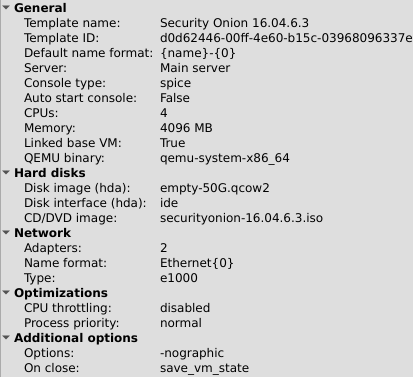
\includegraphics[width=0.6\textwidth]{gns3-so-appliance}
  \caption{Overzicht van de Security Onion GNS3 template}
  \label{fig:gns3-so-appliance}
\end{figure}

\subsection{Simulatie bedrijfsnetwerk}

Een eerste simulatie die ik maakte stelt een typisch bedrijfsnetwerk voor.
Figuur \ref{fig:gns3-simulatie-bedrijf} is een screenshot van dit GNS3 project.

De simulatie bestaat uit een netwerk met 3 Ubuntu hosts (Docker containers) die in verbinding staan met het internet via NAT.
Tussen de Ubuntu hosts en de NAT is er een switch geplaatst.
Deze switch kopieërt alle data die uitgewisseld wordt tussen de Ubuntu hosts en het internet en plaatst deze op een port mirror.
Die port mirror wordt dan gebruikt door Security Onion.

Security Onion is geïnstalleerd als een distributed production deployment bestaande uit een master en forward node. 
Beide nodes zijn met hub management interfaces verbonden aan een switch, die zelf in verbinding staat met een NAT device.
De forward node heeft nog een tweede interface, waar de port mirror op aangeloten is.

De switch die verantwoordelijk is om een port mirror af te leveren bij Security Onion gebruikt de software Open vSwitch.
De built-in switch kan (behalve het aantal poorten en vlans) niet geconfigureerd worden, waardoor een port mirror niet mogelijk is.
De built-in hub werkt wel, maar is geen accurate voorstelling van een port mirror.
Een port mirror dropt alle data die ontvangen wordt.
Een hub stuurt alle ontvangen data op alle andere poorten uit.

Door simpelweg te dubbelklikken op één van de Security Onion nodes opent de volledige desktopomgeving van die machine.
Bij de Ubuntu hosts en Open vSwitch is dit een command prompt en bij \emph{built-in} devices opent er een configuratiescherm van GNS3 zelf.
Dit werkte echter niet meteen.
Het netwerk tussen de GNS3 VM en mijn laptop liet niet toe om andere tcp poorten te gebruiken behalve 22, 80 en 443.
GNS3 heeft een nieuwe poort nodig voor elke command prompt (Telnet) en grafische interface (SPICE) die geopend wordt.
Dit werd opgelost door OpenVPN te installeren op de GNS3 VM en een vpn aan te maken tussen mijn laptop en de GNS3 VM.

De web interface en command line van Security Onion zijn dus beschikbaar via deze desktopomgeving.
Dit is niet ideaal omdat alle inputs en een soort `videostream' van de desktop over een netwerk moet gecommuniceerd worden.
Daarom had ik graag de command line en web interface rechtsreeks beschikbaar op mijn laptop.
Dit kon door ssh verbindingen te openen naar de 2 nodes en de https web interface op poort 443 te openen in een browser.
Hiervoor moest de firewall van Security Onion wel ingesteld worden om het ip van mijn laptop (VPN) toe te laten op poort 22 en 443.

% Evt in bijlage
\begin{figure}[H]
  \centering
  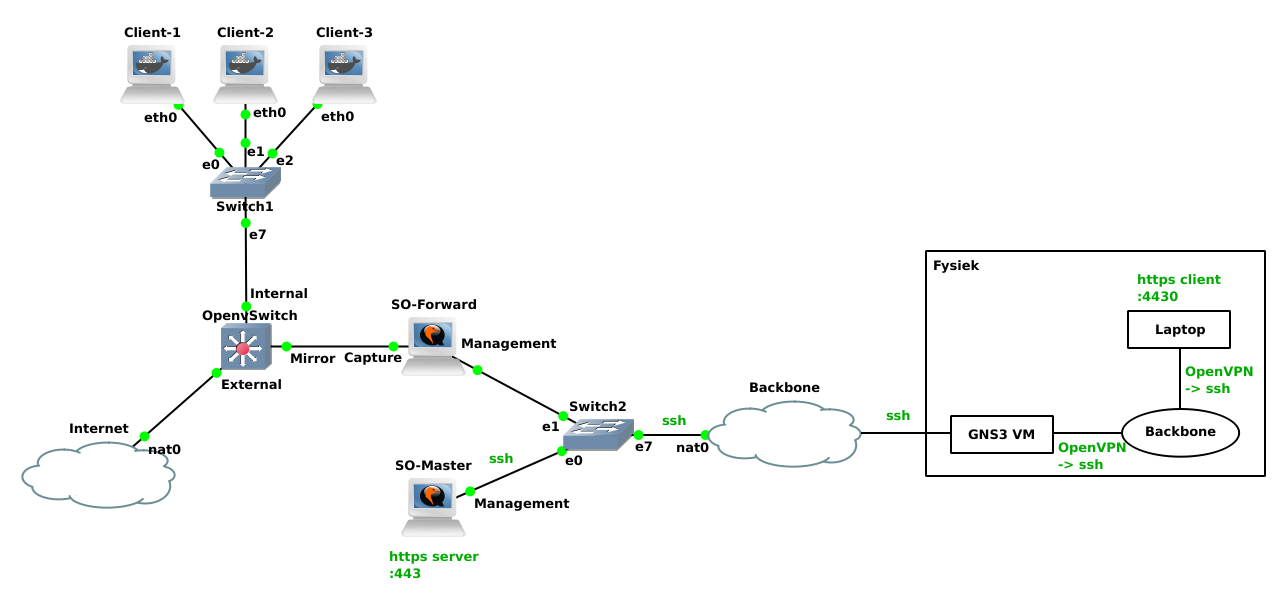
\includegraphics[width=\textwidth]{gns3-simulatie-bedrijf}
  \caption{Screenshot van het bedrijfsnetwerk GNS3 project}
  \label{fig:gns3-simulatie-bedrijf}
\end{figure}

\subsection{Cloud}
Deze simulatie kan ook snel aangepast worden aan een echte port mirror door middel van een GNS3 \emph{built-in} device: de cloud.
De cloud is een device met een kopie van alle netwerk interfaces van de host.
In dit geval is het dus mogelijk om devices in een GNS3 project rechtsreeks in verbinding te zetten met de interfaces van de GNS3 VM.

De server had al één interface, \lstinline|eth0| bedoeld voor het beheren van de VM.
Later werd er een tweede interface toegevoegd, \lstinline|eth1| waar een port mirror op toekwam.
Om snel te testen of een port mirror werkte, werd er een cloud aangemaakt die insgesteld stond om de \lstinline|eth1| interface vrij te geven.
Daarna kon er snel een Ubuntu Docker container mee verbonden worden zoals in figuur \ref{fig:gns3-port-mirror-ubuntu}.
Om de port mirror te bekijken, werd het commando \lstinline|tcpdump -i eth0| op de Ubuntu container uitgevoerd.

\begin{figure}[H]
  \centering
  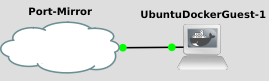
\includegraphics[width=0.4\textwidth]{gns3-port-mirror-ubuntu}
  \caption{De port mirror op de GNS3 VM wordt doorgegeven aan een Ubuntu Docker container}
  \label{fig:gns3-port-mirror-ubuntu}
\end{figure}

Daarna kon hetzelfde systeem terug uitgebouwd worden zoals in de vorige simulatie.
Figuur \ref{fig:gns3-port-mirror-so} is een screenshot van een GNS3 project met dezelfde cloud als in figuur \ref{fig:gns3-port-mirror-ubuntu}, maar met een Security Onion installatie in plaats van een Ubuntu host.

\begin{figure}[H]
  \centering
  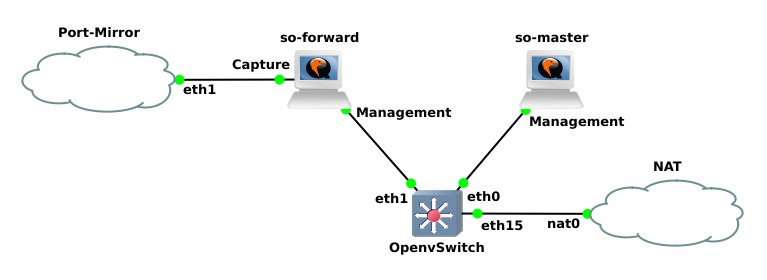
\includegraphics[width=\textwidth]{gns3-port-mirror-so}
  \caption{De port mirror op de GNS3 VM wordt doorgegeven aan een Security Onion installatie}
  \label{fig:gns3-port-mirror-so}
\end{figure}

Met GNS3 clouds kan er echte data aan een simulatieomgeving gekoppeld worden.
GNS3 blijft nog steeds enkel bedoeld voor opstellingen uit te testen, en niet als productieomgeving.
Aspecten waar GNS3 tekort kan komen in vergelijking met een productiesysteem zijn bijvoorbeeld de performantie van netwerkverbindingen en betrouwbaarheid.

\section{Server}
\label{sec:server}
Tijdens mijn stage bij Fluvius kreeg ik een rack-mounted server ter beschikking.
Het was de bedoeling om deze in een serverruimte te plaatsen waar er 2 utp kabels voorzien werden.
Deze 2 kabels werden aangesloten op 2 netwerkinterfaces van de server.
De eerste diende als management interface, op deze interface moest een statisch publiek IPv4 adres geconfigureerd worden.
De tweede interface kreeg een port mirror van een netwerk binnen Fluvius.

Deze server configureerde ik eerst op een andere locatie, waar ik fysieke toegang had tot de server.
Eerst zorgde ik dat het host OS geïnstalleerd was, de netwerkconfiguratie aangepast was en toegang op afstand beschikbaar was via ssh.
Dan verwijderde ik de tijdelijke internetverbinding, stelde ik het statisch publiek ip adres in en testte of dit werkte.
Ten slotte werd deze server geïnstalleerd in de serverruimte, waarna ik fysieke toegang verloor.
De server moest altijd operationeel blijven en de toegang op afstand mocht nooit verloren gaan.

\chapter{Ontwikkelen van een aangepast systeem}
% Proberen schema hier te verwerken
\section{Motivatie}
Na het bekijken van de opnames van enkele presentaties van de Security Onion Conference 2019, bemerkte ik dat er veel mensen proberen externe tools te integreren met Security Onion.
\autocite{so:conference-2019}
Vaak is het doel om in de eerste plaats meer informatie te verzamelen aan de hand van bijvoorbeeld het raadplegen van externe bronnen.
Daarna moet die informatie centraal beschikbaar gesteld worden in een tool als Kibana.

\section{Gebruikte technologie\"en}
\subsection{Debian}
Heel dit systeem is aanwezig op de server eerder besproken in sectie \ref{sec:server}.
In de eerste plaats was er een OS nodig om dit systeem op uit te voeren.

In de keuze van besturingssysteem waren 2 zaken belangrijk.
Het OS moest zeer stabiel zijn, het mocht nooit crashen tijdens het ontwikkelen of uitvoeren van dit systeem.
Daarnaast moest ik altijd de toegang op afstand bewaren.
Omwille van deze redenen koos ik de huidige \emph{stable} branch van Debain: Debian Buster.

\subsection{Docker}
Docker is een verzameling van tools voor het beheren van software containers.
Deze containers zijn applicaties gebundeld met al hun dependencies en configuratie.
Docker is beschikbaar voor enkele verschillende omgevingen, maar voor dit systeem wordt enkel de Linux versie gebruikt.

Docker gebruikt enkele Linux kernel features, vooral Linux namespaces die toelaten om zaken zoals bestandssystemen en de netwerk stack te isoleren.
Dit zorgt ervoor dat Docker containers een volledig andere installatie van Linux kunnen bevatten, het enige wat hetzelfde blijft is de achterliggende Linux kernel.

Dit isolatie systeem zorgt ervoor dat er enkele handige features aanwezig zijn in Docker.
Zo kunnen bestanden, mappen en zelfs Unix sockets gelinkt worden tussen host en container.
Ook kunnen tcp of udp poorten geforward worden naar interfaces van de host en kunnen er ip netwerken gemaakt worden tussen verschillende containers en de host.

Docker kan door softwareontwikkelaars gebruikt worden om hun applicaties samen met alle nodige libraries en andere dependencies, als 1 pakket te publiceren.
Deze applicaties kunnen dan gedownload worden als een Docker image.

% Docker logo

% Evt Dockerfiles tonen

\subsubsection{Dockerfiles}

\autocite{docker:containers}

\subsubsection{Docker compose}
% Github repo presenteren
% Indien het overzichtelijk gebruikt wordt, tool om het volledige systeem mee te ontwerpen
% Compose files tonen

Docker kan ook gebruikt worden bij het ontwikkelen van systemen die bestaan uit meerdere applicaties.
Een typisch voorbeeld hiervan is een webserver en een database.
De http poort van de webserver container wordt dan geforward naar de host en de database container is bereikbaar via een intern netwerk waar beide containers mee verbonden zijn.

Zo'n soort configuraties worden vergemakkelijkt met Docker compose.
Aan de hand van een \lstinline|docker-compose.yml| file en de command-line tool \lstinline|docker-compose| kunnen applicaties ontwikkelt worden die uit meerdere containers bestaan.
\autocite{docker:compose}

Figuur \ref{fig:compose-web-example} is de inhoud van een voorbeeld \lstinline|docker-compose.yml| file van een webserver en een database.
De image voor de web container wordt gebouwd aan de hand van de \lstinline|Dockerfile| in de map \lstinline|web|.
Tcp poort 80 op elke interface van de host wordt geforward naar poort 80 op de interface van de web container.
De image van de MariaDB database wordt opgehaald van een repository zoals Docker Hub.
Deze MariaDB image is zo gemaakt dat het enkel omgevingsvariabelen herkent om makkelijk een nieuwe database en gebruiker aan te maken.

\begin{figure}[H]
  \begin{lstlisting}
version: '3.7'
services:
  web:
    build: web
    ports:
      - 80:80
    depends_on:
      - db
  db:
    image: mariadb:latest
    environment:
      MYSQL_ROOT_PASSWORD: randomized
      MYSQL_RANDOM_ROOT_PASSWORD: 'yes'
      MYSQL_DATABASE: web
      MYSQL_USER=web
      MYSQL_PASSWORD=web
  \end{lstlisting}
  \caption{Voorbeeld van een \lstinline|docker-compose.yml| file voor een webserver en database}
  \label{fig:compose-web-example}
\end{figure}

Dit systeem bestaat bijna volledig uit Docker containers die beheerd worden met Docker compose.
Er zijn meerdere YAML files aanwezig, 1 voor elke applicatie.
Figuur \ref{fig:compose-so-poc-files} is een overzicht van al deze files.
Het bestand \lstinline|compose| is een wrapper script voor \lstinline{docker-compose} die al deze bestanden correct combineert met meerdere \lstinline|-p| flags.

\begin{figure}[H]
  \begin{lstlisting}
.
|- compose
|- docker-compose.misp.yml
|- docker-compose.netdata.yml
|- docker-compose.ntop.yml
|- docker-compose.so-manager.yml
|- docker-compose.so-vm.yml
|- docker-compose.thehive.yml
|- docker-compose.yml
|- ...
  \end{lstlisting}
  \caption{Alle relevante Docker compose bestanden in het so-poc project}
  \label{fig:compose-so-poc-files}
\end{figure}

\subsection{Libvirt}
% logo
De meeste applicaties worden uitgevoerd in docker containers, op 1 na: Security Onion.
Security Onion is niet het meest stabiele systeem om altijd toegang te hebben op afstand, omwille van het regelmatig herstarten tijdens de configuratie en voorgeïnstalleerde firewall.
Om deze toegang zeker niet te verliezen, besloot ik om Security Onion te virtualiseren.

Libvirt is een open source toolkit voor het beheren van virtuele machines voor Linux, BSD en OSX.
Libvirt zelf kan geen virtuele machines uitvoeren, maar kan samen werken met QEMU en KVM om een volledige hypervisor te vormen.
QEMU is een command-line applicatie voor het emuleren en virtualiseren van \emph{machines}.
Eén van de features van QEMU is om de KVM (Kernel-based Virtual Machine) technologie van de Linux kernel te gebruiken om performante virtuele machines te creëren.

Libvirt definieert virtuele machines in XML documenten die gevalideerd worden aan de hand van XML schema's.
Het aanmaken en aanpassen van virtuele machines wordt echter meestal gedaan met een GUI tool zoals \lstinline|virt-manager|.
Soms kan het wel nodig zijn om deze XML files handmatig te bewerken, omdat QEMU zodanig veel opties heeft.
\autocite{libvirt:docs}

Het GUI programma \lstinline|virt-manager| hoeft niet op de server zelf geïnstalleerd te zijn, maar kan ook op afstand werken over een ssh verbinding.
% Screenshot virt-manager

% Uitleggen wat een hypervisor is en bekende alternatieven zoals hyper-v (windows) en virtualbox aanhalen

\section{Intern netwerk}
Vanuit het perspectief van het host besturingssysteem Debian, zijn er 4 interfaces actief.
Deze bestaan uit de management poort, de capture poort, een Libvirt virtueel netwerk en een Docker intern netwerk.

\subsubsection{Management poort}
De management poort is rechtsreeks verbonden met het internet en heeft een statisch publiek ip.
Enkel de poorten voor ssh, http en https zijn actief.
Ssh is beveiligd met een whitelist van geauthoriseerde publieke sleutels, in deze whitelist staan enkel sleutels van mijn persoonlijke apparaten.
De http poort geeft steeds een redirect naar de https poort, tenzij bij het ophalen van nieuwe https certificaten bij \emph{Let's Encrypt}.
Op de https poort zijn alle web services beschikbaar, maar er is steeds een gebruikersnaam en wachtwoord nodig in de vorm van \emph{HTTP basic access authentication} om toegang te krijgen tot deze services.

\subsubsection{Capture poort}
Op de capture poort komt er een port mirror toe.
Toegang tot deze capture poort wordt verspreid naar de verschillende services die deze data nodig hebben.
In Libvirt gebeurt dit via de interface passthrough feature.
In Docker kunnen bepaalde containers toegang krijgen tot het `host net', waar ze toegang hebben aan de capture poort.

\subsubsection{Libvirt virtueel netwerk}
In Libvirt is er 1 virtueel netwerk aangemaakt: \lstinline|192.168.101.0/24|.
In dit netwerk zijn 2 hosts aanwezig: het host besturingssysteem met ip \lstinline|192.168.101.1| en de Security Onion vm met ip \lstinline|192.168.101.2|.
Op deze interface wordt er NAT toegepast, zodat de Security Onion vm externe netwerken zoals het internet kan bereiken via het publieke ip van de management interface.

Dit netwerk werd aangemaakt met de tool \lstinline|virt-manager|.
De XML definitie van dit netwerk is zichtbaar in figuur \ref{fig:libvirt-network-xml}.

\begin{figure}[H]
  \begin{lstlisting}[language=XML]
<network connections="1">
  <name>security-onion</name>
  <uuid>ee6b5b32-fab8-4103-9f49-9d02be6be3d7</uuid>
  <forward mode="nat">
    <nat>
      <port start="1024" end="65535"/>
    </nat>
  </forward>
  <bridge name="virbr1" stp="on" delay="0"/>
  <mac address="52:54:00:87:3d:93"/>
  <domain name="security-onion"/>
  <ip address="192.168.101.1" netmask="255.255.255.0">
  </ip>
</network>
  \end{lstlisting}
  \caption{XML definitie van het Libvirt virtueel netwerk}
  \label{fig:libvirt-network-xml}
\end{figure}

\subsubsection{Docker compose netwerk}
In het docker-compose project is er 1 netwerk gedefinieerd.
Zie figuur \ref{fig:docker-compose-network} voor deze definitie.

Dit netwerkt hangt af van de omgevingsvariabele \lstinline|DOCKER_SUBNET|, gedefinieerd in het bestand \lstinline|.env|.
In dit bestand staat er \lstinline|DOCKER_SUBNET=192.168.100.0/24|.
Het netwerk is dus \lstinline|192.168.100.0/24|, de host neemt het eerste beschikbare adres \lstinline|192.168.100.1| aan.
Docker voorziet alle containers in dit netwerk van een dynamisch ip.
Dit is geen Implementatie van DHCP, maar simpelweg de Docker daemon die een ip adres toekent aan elke container die opstart.
Docker zorgt er ook voor dat de containers elkaar kunnen vinden via DNS lookups van de naam van een Docker compose service. 

\begin{figure}[H]
  \begin{lstlisting}
networks:
  default:
    ipam:
      driver: default
      config:
        - subnet: ${DOCKER_SUBNET}
  \end{lstlisting}
  \caption{Netwerk sectie van het bestand \lstinline|docker-compose.yml|}
  \label{fig:docker-compose-network}
\end{figure}

\section{Structuur project}
Zoals eerder aangehaald is het systeem ontworpen aan de hand van Docker compose.
Elke service heeft een eigen container en elke volledige applicatie (verzameling van services) heeft een eigen \lstinline|docker-compose.yml| file.
Zo zijn er 6 applicaties: so-vm, so-manager, MISP, TheHive, Ntop en Netdata.

\subsection{Structuur bestanden}
De Docker compose configuratie voor elke configuratie staat in een bestand \lstinline|docker-compose.applicatie.yml| en alle 
Alle bestanden die nodig zijn om een applicatie correct te laten werken zijn aanwezig in een map met de naam van de applicatie, met een submap per service of container.
Een volledig overzicht van deze bestanden staat in figuur \ref{fig:so-poc-structuur-docker-compose-containers}.

Elke submap bevat bestanden die nodig zijn voor het bouwen of configureren van een service.
Meestal bestaat dit uit een Dockerfile en enkele configuratiefiles en/of de broncode van de service.

\begin{figure}[H]
  \begin{lstlisting}
.
|- docker-compose.misp.yml
|- docker-compose.netdata.yml
|- docker-compose.ntop.yml
|- docker-compose.so-manager.yml
|- docker-compose.so-vm.yml
|- docker-compose.thehive.yml
|- docker-compose.yml
|- misp
| |- misp-proxy
| \- web
|- netdata
| |- netdata
| \- netdata-proxy
|- ntop
| |- ntopng
| \- ntop-proxy
|- security-onion
| \- rootfs
|- so-manager
| |- api
| |- gotty
| |- react
| \- so-manager-proxy
|- so-vm
| \- so-vm-proxy
|- thehive
  |- thehive
  |- thehive-proxy-cortex
  \- thehive-proxy-thehive
  \end{lstlisting}
  \caption{Overzicht van de structuur van bestanden in het project so-poc}
  \label{fig:so-poc-structuur-docker-compose-containers}
\end{figure}

\subsection{HTTP reverse-proxies}
Merk op dat in figuur \ref{fig:so-poc-structuur-docker-compose-containers} elke applicatie een \emph{proxy} service of container heeft.
Bijna elke applicatie heeft een http interface op 1 van de services binnen de applicatie, elk met een eigen poort.
In plaats van al deze informatie bij te houden, besloot ik om elke applicatie een gelijke http interface te geven.
In elke applicatie is er een service aanwezig met de naam \lstinline|applicatie-proxy| die http verbindingen op poort 80 doorgeeft aan de juiste service binnen de applicatie op de juiste poort.

\subsubsection{Nginx}
% Nginx logo
De software die in elke reverse-proxy wordt gebruikt is Nginx, een open source webserver.
Een van de features van Nginx is de mogelijkheid om als reverse-proxy te werken.
Nginx heeft een officiële Docker image die ik gebruikt heb als basis.
\autocite{nginx:about}

\subsubsection{Voorbeeld}
Als voorbeeld van een proxy service bespreek ik de service \lstinline|so-manager-proxy| in de applicatie \lstinline|so-manager|.

In het bestand \lstinline|docker-compose.so-manager.yml| staat de service \lstinline|so-manager-proxy| gedefinieerd zoals in figuur \ref{fig:proxy-voorbeeld-compose}.
Deze service wacht tot beide \lstinline|so-manager-react| en \lstinline|so-manager-api| opgestart zijn.
De service is geconfigureerd om een nieuwe Docker image te bouwen volgens de inhoud van de map \lstinline|so-manager/so-manager-proxy|.

Die `build' map bevat 2 bestanden: een \lstinline|Dockerfile| en \lstinline|server.conf|, een Nginx configuratiebestand.
Zie figuur \ref{fig:proxy-voorbeeld-dockerfile} voor de inhoud van de \lstinline|Dockerfile| en figuur \ref{fig:proxy-voorbeeld-server-conf} voor de inhoud van \lstinline|server.conf|.

Volgens de \lstinline|Dockerfile| is de image gebaseerd op de laatste versie van de officiële Nginx Docker image, maar wordt de default configuratie verwijderd en in de plaats ervan het bestand \lstinline|server.conf| gebruikt.
Het bestand \lstinline|server.conf| is de configuratie van de http server van Nginx.
Volgens deze configuratie is de server actief op poort 80.
Enkel wanneer de \lstinline|Host| header gelijk is aan \lstinline|so-manager-proxy|, wordt een http request doorgegeven aan \lstinline|http://so-manager-react| of \lstinline|http://so-manager-api|, afhankelijk van het pad in de url.

\begin{figure}[H]
  \begin{lstlisting}
services:
  so-manager-proxy:
    build: so-manager/so-manager-proxy
    depends_on:
      - so-manager-react
      - so-manager-api
  ...
  \end{lstlisting}
  \caption{Verkorte inhoud van het bestand \lstinline|docker-compose.so-manager.yml| in so-poc}
  \label{fig:proxy-voorbeeld-compose}
\end{figure}

\begin{figure}[H]
  \begin{lstlisting}
FROM nginx
RUN rm /etc/nginx/conf.d/default.conf
COPY server.conf /etc/nginx/conf.d/
  \end{lstlisting}
  \caption{De inhoud van het bestand \lstinline|so-manager/so-manager-proxy/Dockerfile| in so-poc}
  \label{fig:proxy-voorbeeld-dockerfile}
\end{figure}

\begin{figure}[H]
  \begin{lstlisting}
server {
  listen 80;
  server_name so-manager-proxy;

  # React
  location / {
    proxy_pass http://so-manager-react;
  }

  # Backend api
  location /api/ {
    proxy_pass http://so-manager-api;
  }

  # Nginx status page
  location /stub_status {
    stub_status;
    access_log off;
  }
}
  \end{lstlisting}
  \caption{Verkorte inhoud van het bestand \lstinline|./so-manager/so-manager-proxy/server.conf| in so-poc}
  \label{fig:proxy-voorbeeld-server-conf}
\end{figure}


\subsubsection{Voordelen}
Het feit dat er reverse-proxies gebruikt worden geeft niet alleen overal een gelijke http interface, maar vergemakkelijkt ook de configuratie van andere zaken.
Elke reverse-proxy is ingesteld om \emph{access logs} bij te houden.
Zo kan van elke applicatie de geschiedenis van http sessies opgevraagd worden, in hetzelfde formaat.
Dit spaart veel tijd bij het toevoegen van een nieuwe applicatie.
Daarnaast zijn de reverse-proxies geconfigureerd om enkele statistieken over recente http sessies te tonen op de \lstinline|/stub_status| pagina.
Deze data wordt opgenomen door Netdata.
Opnieuw is het veel gemakkelijker om nieuwe applicaties toe te voegen, aangezien de statistieken overal op dezelfde manier beschikbaar zijn.

\subsubsection{Beveiliging}
Al de http interfaces tot nu toe besproken, zijn enkel intern bereikbaar.
Aangezien de server een publiek ip heeft, moeten alle verbindingen met de server beveiligd worden.
Met ssh is dit al het geval, enkel de public keys van mijn eigen apparaten worden toegelaten.
De publieke http interface moet dus ook geëncrypteerd worden en toegang moet beperkt zijn.

Voor alle applicaties wordt er https voorzien door de service \lstinline|https-portal|.
Deze service of container gebruikt de image https-portal van \url{https://hub.docker.com/r/steveltn/https-portal}.
De service wordt geconfigureerd door enkele omgevingsvariabelen mee te geven.

Alle configuratie van \lstinline|https-portal| is aanwezig in het bestand \lstinline|docker-compose.yml|.
Merk op dat er geen applicatienaam in dit bestand voorkomt, dit is het hoofdbestand.
In figuur \ref{fig:https-portal-compose} staat het onderdeel \emph{services} van dit bestand.

De service \lstinline|https-portal| werkt als reverse-proxy.
Afhankelijk van de \lstinline|Host| header worden http requests doorgegeven aan de reverse-proxy van 1 van de applicaties.
Al deze routes zijn gedefinieerd in de omgevingsvariabele \lstinline|DOMAINS|.
Communicatie met een externe client gebeurt altijd met https (geëncrypteerd) en communicatie met een interne applicatie gebeurt steeds met http (plain text).

Om toegang tot de applicaties te beperken wordt er http(s) basic authentication gebruikt.
Dit is een gebruikersnaam en wachtwoord die op voorhand ingesteld zijn in het \lstinline|.env| bestand.
Bij sommige applicaties is dit echter niet van toepassing omdat ze zelf al authenticatie implementeren (Security Onion, TheHive en MISP).

Het https certificaat wordt aangemaakt met de Certificate Authority (CA) \emph{Let's Encrypt}.
Dit laat \lstinline|https-portal| toe om gratis en volledig automatisch nieuwe certificaten aan te vragen en ze te hernieuwen.

\begin{figure}[H]
  \begin{lstlisting}
services:
  # Public service
  https-portal:
    image: steveltn/https-portal:1
    ports:
      - 80:80
      - 443:443
    depends_on:
      - so-vm-proxy
      - so-manager-proxy
      - thehive-proxy-thehive
      - thehive-proxy-cortex
      - ntop-proxy
      - netdata-proxy
      - misp-proxy
    restart: always
    environment:
      WEBSOCKET: 'true'
      DOMAINS: '
        ${AUTH_USER}:${AUTH_PASS}@sopoc.duckdns.org -> http://so-manager-proxy,
        so-sopoc.duckdns.org -> http://so-vm-proxy,
        thehive-sopoc.duckdns.org -> http://thehive-proxy-thehive,
        cortex-sopoc.duckdns.org -> http://thehive-proxy-cortex,
        ${AUTH_USER}:${AUTH_PASS}@ntopng-sopoc.duckdns.org -> http://ntop-proxy,
        ${AUTH_USER}:${AUTH_PASS}@netdata-sopoc.duckdns.org -> http://netdata-proxy,
        misp-sopoc.duckdns.org -> http://misp-proxy
      '
      STAGE: 'production'
  \end{lstlisting}
  \caption{Definitie van de service https-portal in het bestand \lstinline|docker-compose.yml| in so-poc}
  \label{fig:https-portal-compose}
\end{figure}

\section{Security Onion}
\subsection{Installatie}
Security Onion werd dus geïnstalleerd in een Libvirt/Qemu/KVM virtuele machine.
De vm is bereikbaar op het ip adres \lstinline|192.168.101.2|.
Deze installatie van Security Onion is een Standalone Production Mode installatie, bestaande uit 1 master node.

De vm heeft 2 netwerk interfaces, een management interface met ip \lstinline|192.168.101.2| en een capture interface waar de port mirror op toekomt.
De port mirror van de host wordt door Libvirt doorgevoerd (passthrough) naar de vm.

De combinatie van de RAID controller en de harde schijven aanwezig in de server resulteerde in minstens 2 logische schijven.
Daarom heb ik 1 schijf toegewezen aan de Debian host en de andere aan de Security Onion vm.
Beide logische schijven zijn RAID-5 arrays.

\subsection{Proxy}
De web interface van Security Onion omvat Squert, Kibana en CyberChef.
De verbinding van een externe client met deze web interface verloopt via het Docker compose netwerk.

Een web browser opent een https verbinding met de \lstinline|https-portal| service.
\lstinline|https-portal| opent een http verbinding met de service \lstinline|so-vm-proxy|.
Ten slotte opent \lstinline|so-vm-proxy| een https verbinding met de Security Onion vm.

De Docker compose service of container \lstinline|so-vm-proxy| is dus een reverse http proxy naar het ip \lstinline|192.168.101.2|.
Omdat Security Onion enkel https aanbied, wordt er een \emph{downgrade} uitgevoerd op deze https verbinding.
De https verbinding wordt dus een http verbinding voor intern gebruik in de Docker compose omgeving.

\section{Web app}
\subsection{React}
% Javascript framework
% States beheren enz, uitleg overnemen van docs
% Material ui library
% dir tree, uitleggen hoe project functioneert
% Homepage en query page
\subsection{Vibe.d}
% Korte omschrijving dlang als general purpose compiled lang
% vibe-d als web framework die toe laat om rest servers en clients te maken
% Werking backend

\section{TheHive}
\subsection{Cortex}
\section{MISP}
\section{Ntop}
\section{Netdata}

\section{Passive os fingerprinting}
% Voordien uitleggen enterprise netwerk met internet en afgesloten netwerk.
Tijdens het uitbreiden van dit systeem heb ik geprobeerd om het besturingssysteem van hosts op een netwerk te bepalen door enkel het netwerkverkeer te analyseren.
Deze uitbreiding was gefocust voor gebruik in een volledig afgesloten netwerk.
\subsection{TCP/IP stack}
In een TCP/IP stack zijn er enkele parameters die niet bepaald worden door de specificatie, maar door de implementatie mogen ingevuld worden.
Voorbeelden van deze parameters zijn de initiële TTL (Time to live) van het IP protocol en de window size van het TCP protocol.
\autocite{wikipedia:fingerprinting}

Elke implementatie van een TCP/IP stack heeft zo een unieke \emph{fingerprint} bestaande uit deze variabele parameters.
Omdat de TCP/IP stack deel is van het besturingssysteem, kunnen deze fingerprints gebruikt worden om het besturingssysteem te bepalen van hosts die communiceren met TCP.
Bij embedded devices kan de fingerprint zelfs eigen zijn aan het apparaat zelf.

\subsubsection{p0f}
p0f is een command-line tool die gebruikt kan worden om het besturingssysteem te bepalen van hosts aan de hand van TCP/IP stack fingerprinting.
De tool kan ofwel met live netwerkverkeer werken door op een interface te capteren, of het kan een pcap file analyseren.

Bij het uitvoeren van analyses kon p0f gebruikt worden om een idee te krijgen welke soort devices geassocieerd zijn met bepaalde ip adressen.
Dit kan bijvoorbeeld gedaan worden door een tcp sessie tussen 2 hosts te vinden in Kibana, de link naar CapMe openen en daar het pcap bestand te downloaden.
Daarna kan p0f uitgevoerd worden op de pcap file met de \lstinline|-r| optie.
Figuur \ref{fig:p0f-so-voorbeeld} is een voorbeeld hiervan.

De resultaten van deze tool zijn soms niet accuraat.
p0f bepaalt het besturingssystem van een host aan de hand van een database die besturingssystemen en hun bijhorende fingerprints bevat.
Deze database is echter al wat verouderd.
Het database bestand \lstinline|p0f.fp| werd het laatst bewerkt in 2016 en heeft bijvoorbeeld geen fingerprint voor Windows 10.
De tool is zo veel minder betrouwbaar als de database niet up to date is.
Omwille van deze reden besloot ik om deze tool niet te integreren in het systeem.

\begin{figure}[H]
  \begin{lstlisting}
$ p0f -r dump.pcap                                           
--- p0f 3.09b by Michal Zalewski <lcamtuf@coredump.cx> ---
...
.-[ 10.170.3.15/49780 -> 10.126.10.151/9877 (syn) ]-
|
| client   = 10.170.3.15/49780
| os       = Windows 7 or 8
| dist     = 1
| params   = none
| raw_sig  = 4:127+1:0:1460:8192,8:mss,nop,ws,nop,nop,sok:df,id+:0
|
`----
...
.-[ 10.170.3.15/49780 -> 10.126.10.151/9877 (syn+ack) ]-
|
| server   = 10.126.10.151/9877
| os       = Windows 7 or 8
| dist     = 6
| params   = none
| raw_sig  = 4:122+6:0:1460:8192,8:mss,nop,ws,nop,nop,sok:df,id+:0
|
`----
...
  \end{lstlisting}
  \caption{Verkorte output van p0f op de pcap dump van een tcp handshake}
  \label{fig:p0f-so-voorbeeld}
\end{figure}

\subsubsection{CapMe}
Wat opviel tijden het uitvoeren van analyses was dat er in CapMe, een web applicatie in Security Onion die pcap files ophaalt en een transcript toont, ook een soort os detectie gebruikt wordt.
In elke transcript wordt het OS van het source ip gegeven samen met een fingerprint in een formaat die lijkt op de fingerprints van p0f.
Ik heb geprobeerd te achterhalen waar deze detectie vandaan komt.
In de broncode van (de Security Onion fork van) CapMe vond ik echter niets terug over de `OS Fingerprint`, het wordt waarschijnlijk op een andere plaats toegevoegd.
Ook in de documentatie van Security Onion of op andere plaaten vondt ik hier niets over terug.

Als voorbeeld heb ik een HTTP sessie uitgekozen tussen een Windows workstation (source) en server (destination).
De workstation is duidelijk een Windows 10 host, bijvoorbeeld te zien door de sting \lstinline|Windows NT 10.0; WOW64;| in de \lstinline|User-Agent| HTTP header.
In figuur \ref{fig:capme-os-detection} detecteert CapMe het besturingssysteem echter als Windows XP/2000.
Voor dezelfde pcap file detecteert p0f het besturingssysteem `Windows NT kernel 5.x'.
Deze kernel werd gebruikt door Windows 2000 en Windows xp.
Beide CapMe en p0f zijn hier dus foutief.

CapMe gebruikt waarschijnlijk dus ook een verouderde database om besturingssystemen te bepalen.

\begin{figure}[H]
  \centering
  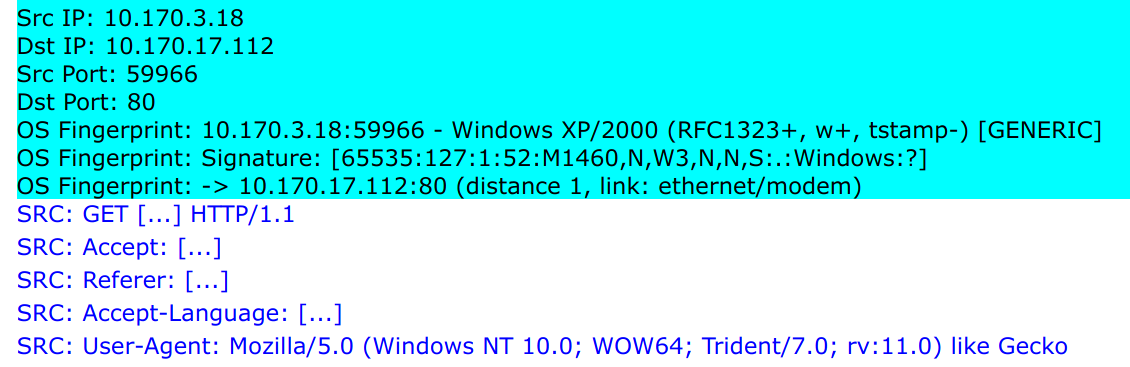
\includegraphics[width=0.6\textwidth]{capme-fingerprint}
  \caption{HTTP request van een Windows 10 workstation in CapMe}
  \label{fig:capme-os-detection}
\end{figure}

\subsection{Fingerbank}
Naast TCP/IP stack fingerprinting bestaan er nog andere manieren om een besturingssysteem of apparaat te herkennen.

In het DHCP protocol zijn er ook enkele parameters die door de implementatie ingevuld worden.
De belangerijkste is de `Parameter request list', die voor bijna elk soort apparaat verschilt.

Http clients geven meestal een \lstinline|User-Agent| header mee met elke http request.
Deze header bevat de browser of andere software die verantwoordelijk is voor de request en soms ook de naam en versie van het besturingssysteem.
De \lstinline|User-Agent| header kan dus geanalyseerd worden om mogelijk het besturingssysteem te achterhalen.

De website \url{https://fingerbank.org/} houdt een lijst bij van apparaten met hun TCP/IP fingerprint, DHCP fingerprint en \lstinline|User-Agent| header.
Fingerbank heeft een REST api waar een combinatie van deze fingerprints ingediend kunnen worden in json formaat, om hopelijk een specifiek soort apparaat en besturingssysteem als antwoord te krijgen.

Toen ik het systeem met OS fingerprinting probeerde uit te breiden, was het doel om het systeem beter te laten werken in een statisch, afgesloten netwerk.
In dit netwerk passeert er geen enkel DHCP pakket.
Ofwel hebben alle apparaten een statisch ip, ofwel worden DHCP paketten niet gerouteerd langs de plaats van de port mirror.

Daarnaast zijn er weinig hosts die http requests versturen en nog minder die een \lstinline|User-Agent| header toevoegen.
Uiteindelijk zijn er enkel twee Windows 10 workstations en een Windows server die zo'n http requests sturen.
Dit is makkelijker manueel te bepalen in Kibana en overbodig om Fingerbank telkens te raadplegen.

Ten slotte is er ook nog de mogelijkheid om TCP/IP stack fingerprints in de dienen.
Aangezien deze van bijna elke host in het netwerk te bepalen zijn, probeerde ik dit uit.
Na wat te experimenteren met scapy en p0f om fingerprints in het juiste formaat in te dienen, bleken de TCP/IP stack fingerprints het minst accurate deel van de Fingerbank database.
Bij de meeste hosts in het afgesloten netwerk kreeg ik als antwoord dat het apparaat en besturingssysteem niet konden bepaald worden.
Mijn eigen desktop werd zelfs herkent als een smartwatch.
Ik bestloot dus om ook Fingerbank niet te gebruiken in het systeem.

Achteraf gezien kon p0f wel een nut gehad hebben in het systeem door de output te parsen en deze toe te voegen aan de logs in de ELK stack.
Toch besloot ik om alternatieven te zoeken die hopelijk accuraater zijn, zonder veel succes.
Ik kan me wel voorstellen dat Fingerbank heel nuttig kan zijn bij het monitoren van bijvoorbeeld een openbaar netwerk.

\section{Visualisatie netwerk layout}
Ik had even geprobeerd om het netwerk die het systeem monitort uit te tekenen in een soort diagram.
Moest ik hierin slagen zou ik het proberen te automatiseren.
Ik ondervond snel enkele problemen die dit bijna onmogelijk maken.

\subsection{Port mirror}
Een port mirror is volledig passief.
Het is dus niet mogelijk om zelf data op het netwerk te plaatsen.
Tools zoals traceroute of nmap die gemaakt zijn om inzicht te krijgen in de layout van een netwerk, kunnen niet gebruikt worden.
De enige mogelijkheid is om het netwerkverkeer te observeren en zo elke host te plaatsen op een diagram.

\subsection{MAC adressen}
Door ARP paketten te bekijken of door zelf destination ip adressen te associëren met destination MAC adressen, kan er een beeld gevormd worden van het laag 2 netwerk waar de port mirror aanwezig is.
In Ntop kunnen alle voorkomende MAC adressen bekeken worden, samen met het aantal geassocieerde ip hosts.
Figuur \ref{fig:visualisatie-netwerk-layout-ntop-mac} is een screenshot hiervan.
De MAC adressen zelf staan niet in de figuur.

\begin{figure}[H]
  \centering
  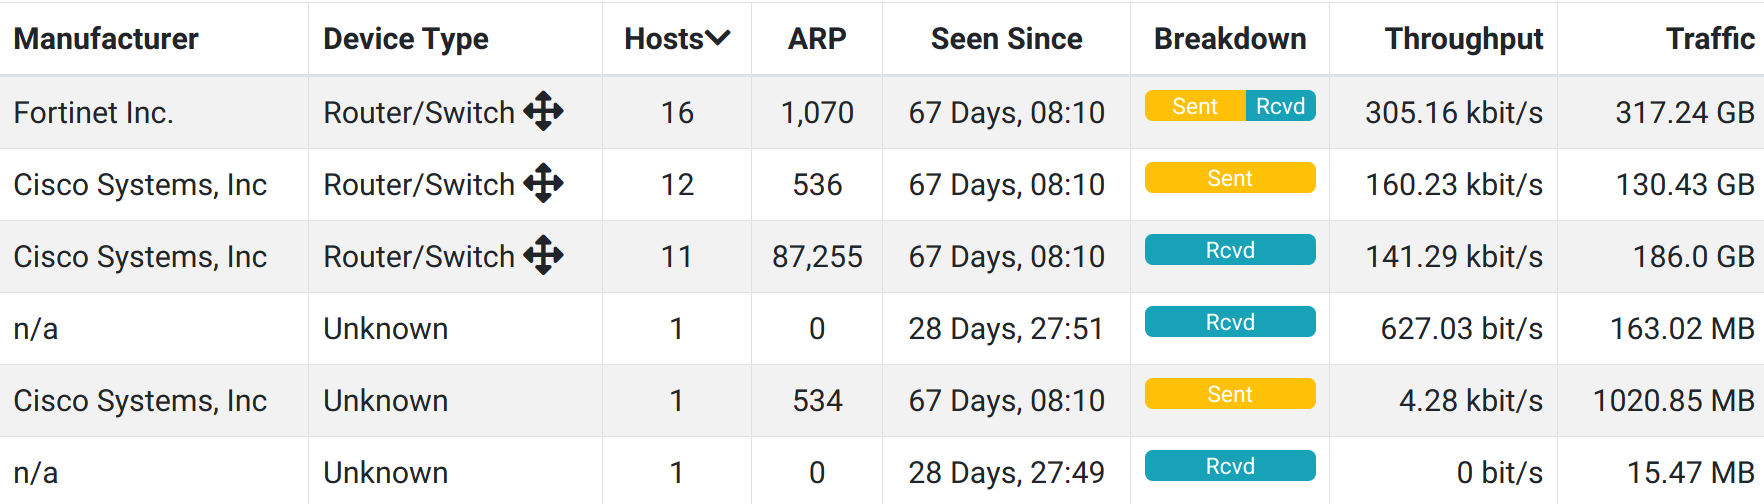
\includegraphics[width=\textwidth]{visualisatie-netwerk-layout-ntop-mac}
  \caption{Screenshot van de `MAC Addresses' pagina in Ntop}
  \label{fig:visualisatie-netwerk-layout-ntop-mac}
\end{figure}

\subsection{IP adressen}
Het is dus mogelijk om een diagram te maken waarop elk ip adres achter één van de mac adressen staat.
Om verder te kunnen bepalen hoe het laag 3 netwerk eruit ziet, is veel moeilijker.

Met een tool zoals traceroute kunnen we duidelijk zien hoe het netwerk eruit ziet, maar dit is een \emph{actieve scan} die we niet kunnen uitvoeren met enkel een port mirror.
De enige optie die ik kan bedenken is om het TTL (Time to live) veld in ip pakketten de bestuderen, om een idee te krijgen van de afstand van een host.

Omdat een simpele actieve scan veel meer informatie oplevert, vond ik het niet nuttig om een tool uit te werken die de weinige informatie beschikbaar door passieve methodes visualiseert.

\chapter{De workflow van een analyst}

% Latex ergens vermelden, github actions

% Reflectie op plaatsen waar het wel nuttig is in een isp
% fingerbank -> wifi netwerk

% Besluit
\chapter*{Besluit}
\addcontentsline{toc}{chapter}{Besluit}
\blindtext

% Bijlagen (niet verplicht)
\chapter*{Bijlagen}
\addcontentsline{toc}{chapter}{Bijlagen}

% Literatuurlijst
\printbibliography
\addcontentsline{toc}{chapter}{Bibliografie}

% Schutblad
\newpage
\thispagestyle{empty}
\mbox{}

% Kaft
\newpage
\thispagestyle{empty}
\mbox{}

\end{document}